\section{A Distributed Build Cache}
\label{sec:motivation}

A distributed build cache enables a team of developers and/or a continuous
integration (CI) system to reuse the build artefacts between several builds.
Such a facility is provided by modern build tools such as Gradle~\cite{Gradle}
and Bazel~\cite{Bazel}, which can store and retrieve build artefacts from cloud
storage services such as Amazon S3 or Google Cloud Storage. Consider the
challenge of building a distributed build cache for OCaml packages. Let us
assume that the builds are reproducible -- that is, independent builds of the same source
files yield the same artefact. In addition to storing the artefacts, it would
be useful to gather statistics about the artefacts such as creation time, last
accessed time and number of cache hits. Such information may be used in the
cache eviction policy or replicating artefacts across several sites for
increased availability. While an artefact itself is reproducible, care must be
taken to ensure that the statistics are consistent. For the sake of exposition,
we will assume that all the build hosts use the same operating system and
compiler version.

\subsection{Mergeable types}

Let us build this distributed cache using \name, implementing in OCaml. At its
heart, \name is a distributed key-value store. The keys in \name are
\emph{paths}, represented as list of strings. The values are algebraic data
types equipped a merge function that reconciles conflicting updates. In this
example, we will use the following schema:
\lstinline[breaklines=true]{[<pkg_name>; <version>; <kind>; <filename>]} for
the keys, where |<kind>| is either |lib| indicating binary artefact or
|stats| indicating statistics about the artefact. The value type is given
below:
\begin{lstlisting}[language=caml]
type timestamp = float
type value =
	| B of bigarray  (*binary artefact*)
	| S of timestamp (*created*) * timestamp (*last accessed*)
	     * int (*hits*)
\end{lstlisting}

\begin{wrapfigure}{r}{0.45\textwidth}
	\vspace{-0.8cm}
	\centering
	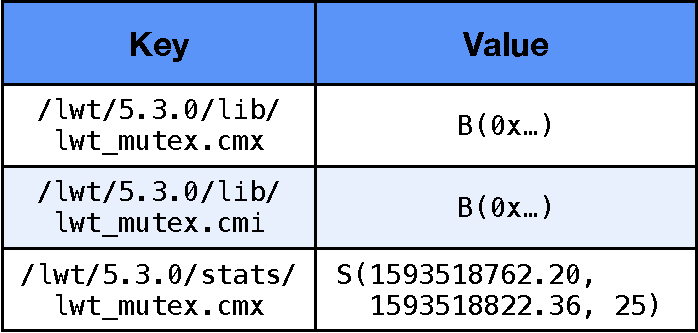
\includegraphics[scale=0.45]{figures/buildcache}
	\caption{A slice of the build cache key-value store.}
	\label{fig:buildcache}
	\vspace{-2.0cm}
\end{wrapfigure}
The value is either a binary artefact or a statistics triple.
Figure~\ref{fig:buildcache} shows the slice of the build cache key-value store.
The cache stores the artefacts (|cmx| and |cmi| files) produced as a result of
compiling the source file |lwt_mutex.ml| from the package |lwt| version
|5.3.0|. The build cache also stores the statistics for every artefact. The
example shows that the |lwt_mutex.cmx| was accessed 25 times. When several
developers and/or CI pipelines are running concurrently on different hosts,
they may attempt to add the same artefact to the store, or, if the artefact is
already present, retrieve it from the cache and update the corresponding
artefact statistics. It would be unwise to synchronize across all of the hosts
for updating the store, and suffer the latency hit and potential
unavailability. Hence, \name only writes an update to one of the replicas. The
replicas asynchronously share the updates between each other, and resolve
conflicting updates using used-defined three-way merge function. The merge
function for the build cache is given below.

\begin{lstlisting}[language=caml, numbers=left]
let merge (lca: value option) (v1: value) (v2: value) : value =
  match lca, v1, v2 with
  | None, B a1, B a2 (* no lca *)
  | Some (B _), B a1, B a2 -> assert (a1 = a2); B a1
  | None, S(c1,la1,h1), S(c2,la2,h2) -> (* no lca *)
      S(min c1 c2, max la1 la2, h1 + h2)
  | Some(S(_,_,h0)), S(c1,la1,h1), S(c2,la2,h2)->
      S(min c1 c2, max la1 la2, h1 + h2 - h0)
  | _ -> failwith "impossible"
\end{lstlisting}

The key idea here is that \name tracks the \emph{causal history} of the state
updates such that it is always known what the \emph{lowest common ancestor}
(LCA) state is, if one exists. This idea is analogous to how Git tracks history
with the notion of \emph{branches}. The merge function is applied to the LCA
and the two conflicting versions to determine the new state. In the case of
build cache, since the builds are reproducible, the binary artefacts will be
the same (line 4). The only interesting conflicts are in the statistics. The
merge function picks the earliest creation timestamp, latest last accessed
timestamp, and the sum of the new cache hits since the LCA in the two branches
and the original value at the LCA, if present (lines 5--8).

\begin{wrapfigure}{r}{0.5\textwidth}
	\vspace{-0.9cm}
	\centering
	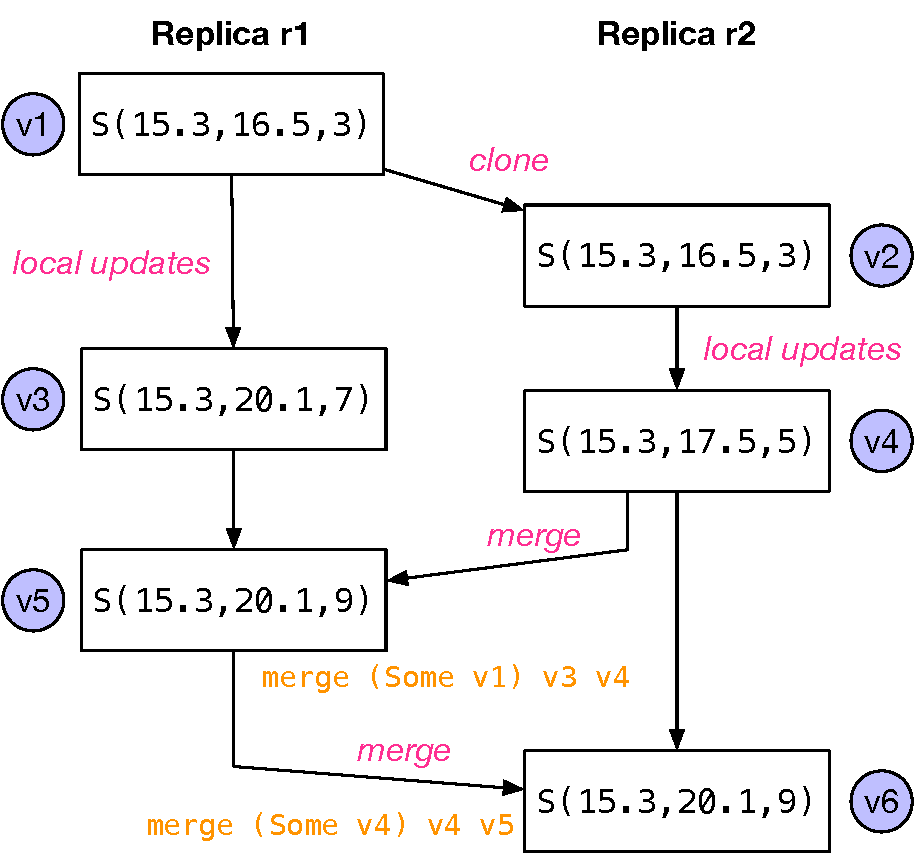
\includegraphics[scale=0.4]{figures/replica_merge}
	\caption{Merging conflicting statistics updates.}
	\label{fig:replica_merge}
	\vspace{-0.8cm}
\end{wrapfigure}
Figure~\ref{fig:replica_merge} shows how the merge function helps reconcile
conflicts. The arrows capture the happens-before relationship between the
states. Assume that replica |r2| starts off by cloning the branch corresponding
to replica |r1|. Subsequently both |r1| and |r2| performed local updates. The
remote updates are reconciled by calling the merge function on each of the
conflicting values. The value |v5| is obtained with merging the values |v3| and
|v4| with |v1| as LCA. Importantly, observe that the cache hit count is |9| in
|v5| which corresponds to the sum of |3| hits in the initial state, |4|
additional hits in |r1| and |2| additional hits in |r2|. At this point, |r1|
has all the changes from |r2|, but the vice-versa is not true. Subsequently,
when |r1| is merged into |r2|, both the replicas have converged.

\begin{figure}%{r}{0.6\textwidth}
	\vspace{-0.5cm}
	\begin{lstlisting}
let compile s (* session *) =
	let ts = Unix.gettimeofday () in
	let lib = ["lwt";"5.3.0";"lib"] in
	let stats = ["lwt";"5.3.0";"stats"] in
	refresh s >>= fun () ->
	read s (lib @ ["lwt_mutex.cmx"]) >>= fun v ->
	match v with
	| None ->
			let (cmx, cmi, o) = ocamlopt "lwt_mutex.ml" in
			write s (lib @ ["lwt_mtex.cmx"]) (B cmx) >>= fun _ ->
			write s (stats @ ["lwt_mutex.cmx"]) (S (ts,ts,0)) >>= fun _ ->
			... (* similarly for cmi and o files *)
			publish s >>= fun _ ->
			return (cmx, cmi, o)
	| Some cmx ->
			read s (stats @ ["lwt_mutex.cmx"]) >>= fun (Some M(c,la,h)) ->
			write s (stats @ ["lwt_mutex.cmx"]) (S (c,ts,h+1)) >>= fun _ ->
			read s (lib @ ["lwt_mutex.cmi"]) >>= fun (Some cmi) ->
			read s (lib @ ["lwt_mutex.o"]) >>= fun (Some o) ->
			... (* update stats for cmi and o file *)
			publish s >>= fun _ ->
			return (cmx, cmi, o)
	\end{lstlisting}
	\caption{Compiling \texttt{lwt\_mutex.ml}.}
	\label{code:compile}
	\vspace{-1cm}
\end{figure}

\subsection{Transactions}

Now that we the mergeable value type for the build cache, let us see how we can
compile |lwt_mutex.ml| using \name. Figure~\ref{code:compile} shows the code
for compiling |lwt_mutex.ml|. In \name, the clients interact with the store in
\emph{isolated} sessions. A session can fetch recent updates using the
|refresh| primitive and make \emph{all} the local updates visible to other
sessions using the |publish| primitive. During |refresh|, any conflicting
updates are resolved using the three-way merge function associated with the
value type.

In order to compile |lwt_mutex.ml|, we first refresh the session to get any
recent updates. Then, we check whether the |lwt_mutex.cmx| file is in the build
cache. If not, the source file is compiled, and the resultant artefacts (|cmx|,
|cmi|, |o| files) and the corresponding entries for updated statistics are
written to the store. Finally, the all the local updates are published.

The all or nothing property of |refresh| and |publish| is critical for the
correctness of this code. Observe that when the artefact is locally compiled,
all the artefacts and their statistics are published atomically. This ensures
that if a session sees the |cmx| file, then other artefacts and their
statistics will also be visible. Thus, \name makes it easy to write highly-available,
complex distributed applications in an idiomatic fashion.
